\documentclass{scrartcl}
\usepackage[utf8]{inputenc}

\title{Der Vielfraß - König der Riesenmarde}
\author{nalcock1 }
\date{February 2021}

\usepackage{natbib}
\usepackage{graphicx}

\begin{document}
\maketitle
\tableofcontents
\newpage

\\
\\
\section{Vielfraß}
Der Vielfraß (Gulo gulo) ist eine Raubtierart aus der Familie der Marder (Mustelidae), die im nördlichen Eurasien und in Nordamerika lebt. Er wird auch als Bärenmarder, Gierling, Giermagen oder Gierschlund bezeichnet. 



\begin{figure}[h!]
\centering
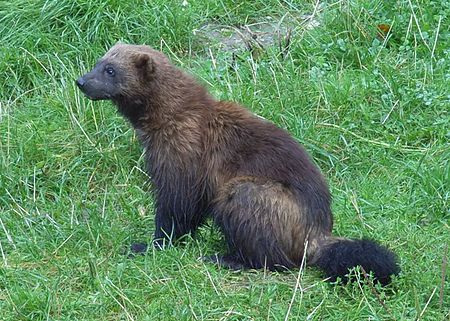
\includegraphics[scale=0.7]{Vielfraß}
\caption{Vielfraß (Gulo gulo)}
\label{Vielfraß (Gulo gulo)}
\end{figure}

\section{Herkunft des Namens}
Die Herkunft des Tiernamens Vielfraß (von mittelhochdeutsch vilfrāz, „Gefräßiger“, als Name des ‚Bärenmarders‘, gelegentlich auch der ‚Hyäne‘; althochdeutsch bereits vilifrāz)[1] ist nicht sicher zu deuten. Die etablierte Annahme ist, dass er – über den hansischen Fellhandel des 15. Jahrhunderts in deutsches Gebiet gekommen – eine volksetymologische Umbildung des altnorwegischen fjeldfross sei, was so viel wie ‚Felsenkater‘ oder „Bergkater“ bedeutet[2] und die Erzählungen über seine Gefräßigkeit erst durch den umgedeuteten Tiernamen entstanden. Dies wird jedoch gelegentlich bestritten.
\\
Eine andere Vermutung ist, dass das Tier seinen Namen der Eigenschaft verdanke, alles halbwegs Genießbare in die Nähe seines Schlupfwinkels zu schleppen und dort große Vorräte anzulegen.[3] Namen, die auf Gefräßigkeit hindeuten, wahrscheinlich aber auf dem umgedeuteten deutschen Namen „Vielfraß“ beruhen, hat der Vielfraß auch in mehreren anderen Sprachen. Auch die wissenschaftliche Bezeichnung (Gulo gulo) nimmt Bezug auf die gefräßige, nordische Sagengestalt Gulon. In allen modernen skandinavischen Sprachen wird eine dem schwedischen järv analoge Bezeichnung verwendet. Der gebräuchlichste englische Name des Vielfraßes ist „wolverine“. 


\section{Merkmale}
Der Vielfraß ähnelt in seinem Körperbau den Echten Mardern, wird aber deutlich größer. Er erreicht eine Kopf-Rumpf-Länge von 65 bis 105 Zentimetern und eine Schwanzlänge von 17 bis 26 Zentimetern. Mit einem Gewicht von bis zu 32 Kilogramm werden Männchen deutlich schwerer als Weibchen, die 20 Kilogramm erreichen können. Der massive Kopf und die kräftigen Gliedmaßen erwecken einen deutlich kompakteren und kräftigeren Eindruck als bei anderen Mardern. Die Ohren sind relativ klein und der Schwanz ist kurz und buschig. Das lange, dichte Fell ist dunkelbraun oder schwärzlich gefärbt, charakteristisch ist eine gelbliche oder hellbraune Bandzeichnung, die sich von den Schultern über die Seiten des Rumpfes erstreckt und sich über der Schwanzwurzel wieder vereint. 

\section{Verbreitung und Lebensraum}
Der Vielfraß ist über die Taiga- und Tundragürtel der nördlichen Halbkugel verbreitet. Sein heutiges Verbreitungsgebiet umfasst Skandinavien, das nördliche Sibirien, Alaska, weite Teile Kanadas und vereinzelte Populationen im Nordwesten der Vereinigten Staaten. In geschichtlicher Zeit war er auch weiter südlich heimisch, so in Polen und im Baltikum und in etlichen Regionen der Vereinigten Staaten, wo sich sein Verbreitungsgebiet bis Kalifornien und Pennsylvania erstreckte. Aus diesen Gegenden wurde er durch menschliche Bejagung zurückgedrängt.[4] In der Harzer Einhornhöhle wurden Vielfraßknochen aus einer Epoche der Kaltzeit (Glazialfauna) gefunden.[5] Knochen aus früher Zeit wurden auch an vielen Stellen im Alpenraum und umliegenden Landschaften wie den Westkarpaten gefunden, wobei die meisten Fundstellen zwischen 200 und 950 Metern über dem Meer liegen.[6]
Am häufigsten sind Vielfraße in den borealen Nadelwäldern, doch auch in den baumlosen Mooren der Tundra und in Gebirgsregionen sind sie weit verbreitet. 


\section{Lebensweise}
Vielfraße sind vorwiegend nachtaktiv, im Norden ihres Verbreitungsgebietes halten sie während der Polartage und Polarnächte einen alternierenden Rhythmus mit jeweils drei- bis vierstündigen Schlaf- und Aktivitätszeiten. Zur Ruhe ziehen sie sich in Nester zurück, die sie aus Gräsern und Blättern in Höhlen, Felsspalten oder unter gefallenen Bäumen anlegen. Manchmal beziehen sie auch Baue anderer Tiere oder legen Höhlen im Schnee an. Sie sind in erster Linie Bodenbewohner, können aber auch gut klettern und schwimmen. Sie sind nicht sehr schnelle, aber ausdauernde Läufer, die 10 bis 15 Kilometer ohne Pause zurücklegen und in einer Nacht Distanzen bis zu 45 Kilometern bewältigen können. Sie halten keine Winterruhe, wandern im Winter aber manchmal in tiefergelegene oder südlichere Regionen ab.
\\
Wie die meisten Marder leben Vielfraße einzelgängerisch. Sie sind territoriale und markieren ihr Revier oder zumindest ihr derzeitiges Aufenthaltsgebiet mit dem Sekret ihrer Analdrüsen oder mit Urin. Gegenüber gleichgeschlechtlichen Artgenossen sind sie in der Regel intoleranter als gegenüber Vertretern des anderen Geschlechts, das Revier eines Männchens kann sich mit denen mehrerer Weibchen überlappen oder sogar gänzlich überschneiden. Die Reviere sind verhältnismäßig groß und können im Winter 2000 Quadratkilometer (annähernd die Größe des Saarlandes) umfassen.
\\
Der Vielfraß gilt als außergewöhnlich kräftig und angriffslustig und wurde beobachtet, als er Pumas oder Bären vom Riss vertrieb. 

\section{Nahrung}
Im Sommer zeigt der Vielfraß ein ganz anderes Jagdverhalten als im Winter. In der warmen Jahreszeit betätigt er sich vor allem als Aasfresser, sucht aber auch nach Vogeleiern, Baumtrieben und Beeren. Nur selten reißt er junge Rentiere oder Elchkälber, wenn er sie unbewacht antrifft.
\\
Im Winter hat der Vielfraß einen Vorteil gegenüber großen Säugetieren, da er sich auf dem Schnee fast geräuschlos nähern kann, ohne einzusinken. Seine Hauptbeute sind in dieser Zeit Schneehasen, Mäuse, Eichhörnchen und Schneehühner, gelegentlich auch Rentiere[7], junge Elche und sogar Luchse. 

\section{Fortpflanzung}

Die Paarung erfolgt in den Monaten April bis Juli. Bedingt durch eine Keimruhe beginnt die eigentliche Tragzeit erst zwischen November und März. Nach rund 30- bis 40-tägiger effektiver Trächtigkeitsdauer bringt das Weibchen zwei bis vier Jungtiere zur Welt. Es legt oft eine Schneehöhle an, in der die Jungtiere ihre ersten Lebenswochen verbringen. Neugeborene sind schneeweiß, blind und wiegen rund 90 bis 100 Gramm. Sie werden acht bis zehn Wochen gesäugt und verlassen die Mutter im Herbst. Nach einem Jahr erreichen sie ihre volle Größe, nach zwei bis drei Jahren werden sie geschlechtsreif. Die Lebenserwartung in freier Wildbahn beträgt acht bis zehn Jahre, in menschlicher Obhut können sie zu 17 Jahren alt werden. 
\\
\begin{center}}
 Fortpflanzungsformel
  \end{center}
\begin{equation}
    x_t=\frac{1}{\omega_t}(\frac{x_{t-1}-\omega_{t-1}}{\eta*\epsilon})\\
\end{equation}



\section{Mensch und Vielfraß}

Früher wurden Schauergeschichten über die Gefräßigkeit des Vielfraßes verbreitet: So berichtet Brehms Tierleben (allerdings mit Skepsis), dass er sich an Aas (nach einer alten Erzählung von Conrad Gessner sogar an einer Leiche) vollfresse und sich dann zwischen engstehenden Bäumen durchzwänge, um den Darminhalt möglichst rasch loszuwerden und sogleich weiterzufressen. Großen Tieren springe der Vielfraß auf den Rücken, um sie in den Nacken zu beißen, bis sie stürzen.[8] Auch in Zedlers Universallexikon wird 1746 der Vielfraß erwähnt und 1771 in der Göttinger Dissertation[9] von Samuel Gottlieb Vogel.[10]
\\
Verfolgung
\\
Die Bejagung des Vielfraßes und die damit verbundene Verkleinerung seines Verbreitungsgebietes hat zwei Gründe. Zum einen sieht man ihn als Nahrungskonkurrenten, Rentierzüchter fürchten ihn, da er manchmal ihr Vieh reißt. Aus diesem Grunde wurde er in Skandinavien bis in die jüngste Zeit gejagt. Außerdem dringt er manchmal auf der Suche nach Nahrung in Häuser ein, wo er den strengen Geruch seines Analdrüsensekretes verbreitet.
\\
Der zweite Grund für die Jagd war der Vielfraßpelz. Er galt früher als wertvoll, spielt heute aber im kommerziellen Pelzhandel keine Rolle mehr. Von arktischen Völkern wird er als Kälteschutz geschätzt. 

\section{Bestand und Schutz}

Im nördlichen Mitteleuropa ist die Art ausgestorben, in Norwegen gibt es nur mehr eine kleine Population von 120 bis 150 Tieren, die streng geschützt ist. Die schwedische Vielfraßpopulation war so gut wie ausgestorben, wurde aber 1969 unter Schutz gestellt und konnte sich in den letzten Jahren erholen. Im Jahr 2012 lebten zwischen 668 und 835 Tiere, die hauptsächlich in Lappland und vereinzelt in Dalarna vorkommen.[11] In Finnland hat sich der Bestand zwischen 1991 und 2007 fast verdoppelt und wird derzeit auf 150 bis 170 Individuen geschätzt.[12]
\\
Im östlichen und südlichen Kanada sind Vielfraße ausgerottet, ebenso im größten Teil des Kerngebietes der Vereinigten Staaten, wo nur mehr vereinzelte Reliktpopulationen vorkommen. In Nordasien, dem nördlichen Kanada und Alaska sind sie noch häufiger, insgesamt gelten sie laut Weltnaturschutzunion IUCN als nicht gefährdet („Least Concern“). In Deutschland sind nach dem Bundesnaturschutzgesetz und der Bundesartenschutzverordnung Handel und Einfuhr von europäisch wild lebenden Populationen bzw. deren Erzeugnisse verboten, um die Bejagung in den verbliebenen natürlichen Lebensräumen nicht zu begünstigen.[13] 

\begin{table}
    \centering
    \caption{Vielfraßbestand nach Kontinent und Gefährdungsstatus}
    \\
    \begin{tabular}{l|l|l}
         Asien & 20000 & low\\
         Afrika & 5000 & low\\
         Europa & 1500 & medium\\
         Americas & 300 & high\\
         Ozeanien & 15 & extreme\\
    \end{tabular}
\end{table}

\section{Systematik}

Die systematischen Beziehungen des Vielfraßes zu anderen Mardern sind nicht restlos geklärt. Aufgrund von Besonderheiten im Körperbau wird er manchmal in eine eigene Unterfamilie, Guloninae, gestellt. Genetische Untersuchungen stützen diese Sichtweise aber nicht, sondern ordnen ihn in die Martinae ein, möglicherweise ist sogar die Gattung der Echten Marder (Martes) ohne den Vielfraß paraphyletisch. Demnach könnte dieser ein enger Verwandter des nordamerikanischen Fischermarders sein. 

\section{Literatur}

    \item Ronald M. Nowak: Walker’s mammals of the world. 6. Auflage. Johns Hopkins University Press, Baltimore 1999, ISBN 0-8018-5789-9 (englisch).
    \item John J. Flynn, John A. Finarelli, Sarah Zehr, Johnny Hsu, Michael A. Nedbal: Molecular phylogeny of the Carnivora (Mammalia). Assessing the impact of increased sampling on resolving enigmatic relationships. In: Systematic Biology. Band 54 (2), 2005, doi:10.1080/10635150590923326, S. 1–21.
    \item  Robert M. Inman, Audrey J. Magoun, Jens Persson, Jenny Mattisson: The wolverine's niche: linking reproductive chronology, caching, competition, and climate. In: Journal of Mammalogy 93 (3), 2012, doi:10.1644/11-MAMM-A-319.1, S. 634–644.

\bibliographystyle{plain}

\end{document}
